% Created by tikzDevice version 0.10.1 on 2020-02-15 16:19:28
% !TEX encoding = UTF-8 Unicode
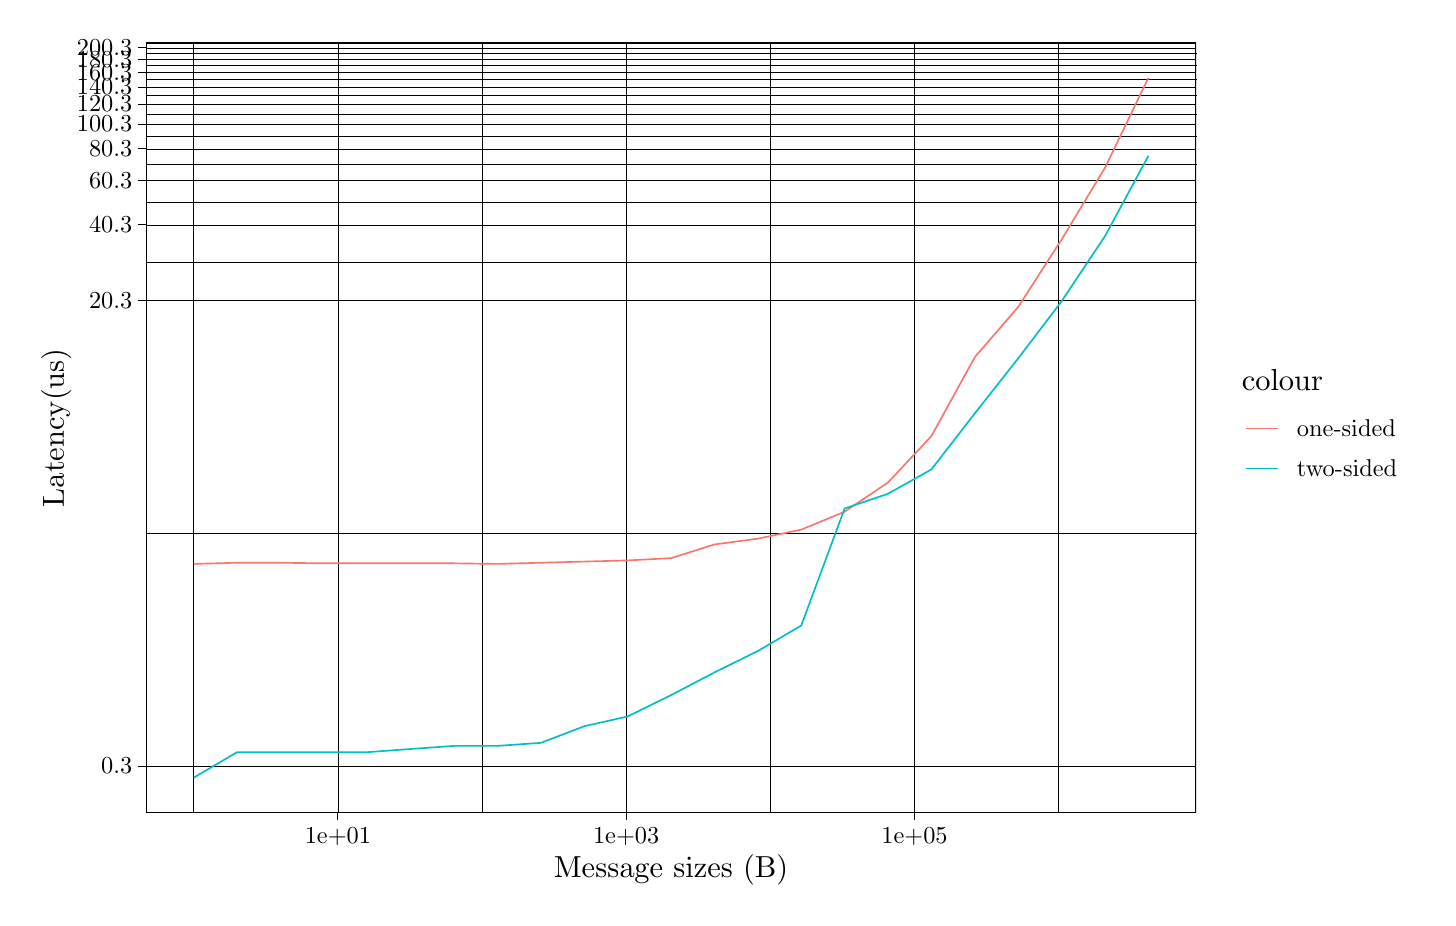
\begin{tikzpicture}[x=1pt,y=1pt]
\definecolor{fillColor}{RGB}{255,255,255}
\path[use as bounding box,fill=fillColor,fill opacity=0.00] (0,0) rectangle (505.89,314.37);
\begin{scope}
\path[clip] (  0.00,  0.00) rectangle (505.89,314.37);
\definecolor{drawColor}{RGB}{255,255,255}
\definecolor{fillColor}{RGB}{255,255,255}

\path[draw=drawColor,line width= 0.6pt,line join=round,line cap=round,fill=fillColor] (  0.00,  0.00) rectangle (505.89,314.37);
\end{scope}
\begin{scope}
\path[clip] ( 42.76, 30.72) rectangle (422.22,308.87);
\definecolor{fillColor}{RGB}{255,255,255}

\path[fill=fillColor] ( 42.76, 30.72) rectangle (422.22,308.87);
\definecolor{drawColor}{RGB}{0,0,0}

\path[draw=drawColor,line width= 0.0pt,line join=round] ( 42.76,131.67) --
	(422.22,131.67);

\path[draw=drawColor,line width= 0.0pt,line join=round] ( 42.76,229.45) --
	(422.22,229.45);

\path[draw=drawColor,line width= 0.0pt,line join=round] ( 42.76,251.17) --
	(422.22,251.17);

\path[draw=drawColor,line width= 0.0pt,line join=round] ( 42.76,264.93) --
	(422.22,264.93);

\path[draw=drawColor,line width= 0.0pt,line join=round] ( 42.76,275.08) --
	(422.22,275.08);

\path[draw=drawColor,line width= 0.0pt,line join=round] ( 42.76,283.15) --
	(422.22,283.15);

\path[draw=drawColor,line width= 0.0pt,line join=round] ( 42.76,289.84) --
	(422.22,289.84);

\path[draw=drawColor,line width= 0.0pt,line join=round] ( 42.76,295.57) --
	(422.22,295.57);

\path[draw=drawColor,line width= 0.0pt,line join=round] ( 42.76,300.58) --
	(422.22,300.58);

\path[draw=drawColor,line width= 0.0pt,line join=round] ( 42.76,305.02) --
	(422.22,305.02);

\path[draw=drawColor,line width= 0.0pt,line join=round] ( 60.01, 30.72) --
	( 60.01,308.87);

\path[draw=drawColor,line width= 0.0pt,line join=round] (164.18, 30.72) --
	(164.18,308.87);

\path[draw=drawColor,line width= 0.0pt,line join=round] (268.36, 30.72) --
	(268.36,308.87);

\path[draw=drawColor,line width= 0.0pt,line join=round] (372.54, 30.72) --
	(372.54,308.87);

\path[draw=drawColor,line width= 0.1pt,line join=round] ( 42.76, 47.57) --
	(422.22, 47.57);

\path[draw=drawColor,line width= 0.1pt,line join=round] ( 42.76,215.76) --
	(422.22,215.76);

\path[draw=drawColor,line width= 0.1pt,line join=round] ( 42.76,243.13) --
	(422.22,243.13);

\path[draw=drawColor,line width= 0.1pt,line join=round] ( 42.76,259.21) --
	(422.22,259.21);

\path[draw=drawColor,line width= 0.1pt,line join=round] ( 42.76,270.64) --
	(422.22,270.64);

\path[draw=drawColor,line width= 0.1pt,line join=round] ( 42.76,279.52) --
	(422.22,279.52);

\path[draw=drawColor,line width= 0.1pt,line join=round] ( 42.76,286.77) --
	(422.22,286.77);

\path[draw=drawColor,line width= 0.1pt,line join=round] ( 42.76,292.91) --
	(422.22,292.91);

\path[draw=drawColor,line width= 0.1pt,line join=round] ( 42.76,298.23) --
	(422.22,298.23);

\path[draw=drawColor,line width= 0.1pt,line join=round] ( 42.76,302.92) --
	(422.22,302.92);

\path[draw=drawColor,line width= 0.1pt,line join=round] ( 42.76,307.12) --
	(422.22,307.12);

\path[draw=drawColor,line width= 0.1pt,line join=round] (112.10, 30.72) --
	(112.10,308.87);

\path[draw=drawColor,line width= 0.1pt,line join=round] (216.27, 30.72) --
	(216.27,308.87);

\path[draw=drawColor,line width= 0.1pt,line join=round] (320.45, 30.72) --
	(320.45,308.87);
\definecolor{drawColor}{RGB}{248,118,109}

\path[draw=drawColor,line width= 0.6pt,line join=round] ( 60.01,120.60) --
	( 75.69,121.02) --
	( 91.37,121.02) --
	(107.05,120.81) --
	(122.73,120.81) --
	(138.41,120.81) --
	(154.09,120.81) --
	(169.77,120.60) --
	(185.45,121.02) --
	(201.13,121.44) --
	(216.81,121.86) --
	(232.49,122.68) --
	(248.17,127.63) --
	(263.85,129.72) --
	(279.53,132.98) --
	(295.21,139.46) --
	(310.89,150.03) --
	(326.57,166.79) --
	(342.25,195.31) --
	(357.93,213.46) --
	(373.61,237.82) --
	(389.29,263.76) --
	(404.97,296.23);
\definecolor{drawColor}{RGB}{0,191,196}

\path[draw=drawColor,line width= 0.6pt,line join=round] ( 60.01, 43.37) --
	( 75.69, 52.57) --
	( 91.37, 52.57) --
	(107.05, 52.57) --
	(122.73, 52.57) --
	(138.41, 53.72) --
	(154.09, 54.85) --
	(169.77, 54.85) --
	(185.45, 55.94) --
	(201.13, 61.94) --
	(216.81, 65.49) --
	(232.49, 73.19) --
	(248.17, 81.39) --
	(263.85, 89.13) --
	(279.53, 98.32) --
	(295.21,140.64) --
	(310.89,145.95) --
	(326.57,154.75) --
	(342.25,175.00) --
	(357.93,194.88) --
	(373.61,215.49) --
	(389.29,239.04) --
	(404.97,268.06);
\definecolor{drawColor}{RGB}{0,0,0}

\path[draw=drawColor,line width= 0.6pt,line join=round,line cap=round] ( 42.76, 30.72) rectangle (422.22,308.87);
\end{scope}
\begin{scope}
\path[clip] (  0.00,  0.00) rectangle (505.89,314.37);
\definecolor{drawColor}{RGB}{0,0,0}

\node[text=drawColor,anchor=base west,inner sep=0pt, outer sep=0pt, scale=  0.88] at ( 26.57, 44.75) {0.3};

\node[text=drawColor,anchor=base west,inner sep=0pt, outer sep=0pt, scale=  0.88] at ( 22.17,212.94) {20.3};

\node[text=drawColor,anchor=base west,inner sep=0pt, outer sep=0pt, scale=  0.88] at ( 22.17,240.31) {40.3};

\node[text=drawColor,anchor=base west,inner sep=0pt, outer sep=0pt, scale=  0.88] at ( 22.17,256.39) {60.3};

\node[text=drawColor,anchor=base west,inner sep=0pt, outer sep=0pt, scale=  0.88] at ( 22.17,267.82) {80.3};

\node[text=drawColor,anchor=base west,inner sep=0pt, outer sep=0pt, scale=  0.88] at ( 17.77,276.70) {100.3};

\node[text=drawColor,anchor=base west,inner sep=0pt, outer sep=0pt, scale=  0.88] at ( 17.77,283.95) {120.3};

\node[text=drawColor,anchor=base west,inner sep=0pt, outer sep=0pt, scale=  0.88] at ( 17.77,290.09) {140.3};

\node[text=drawColor,anchor=base west,inner sep=0pt, outer sep=0pt, scale=  0.88] at ( 17.77,295.41) {160.3};

\node[text=drawColor,anchor=base west,inner sep=0pt, outer sep=0pt, scale=  0.88] at ( 17.77,300.10) {180.3};

\node[text=drawColor,anchor=base west,inner sep=0pt, outer sep=0pt, scale=  0.88] at ( 17.77,304.30) {200.3};
\end{scope}
\begin{scope}
\path[clip] (  0.00,  0.00) rectangle (505.89,314.37);
\definecolor{drawColor}{RGB}{0,0,0}

\path[draw=drawColor,line width= 0.3pt,line join=round] ( 40.01, 47.57) --
	( 42.76, 47.57);

\path[draw=drawColor,line width= 0.3pt,line join=round] ( 40.01,215.76) --
	( 42.76,215.76);

\path[draw=drawColor,line width= 0.3pt,line join=round] ( 40.01,243.13) --
	( 42.76,243.13);

\path[draw=drawColor,line width= 0.3pt,line join=round] ( 40.01,259.21) --
	( 42.76,259.21);

\path[draw=drawColor,line width= 0.3pt,line join=round] ( 40.01,270.64) --
	( 42.76,270.64);

\path[draw=drawColor,line width= 0.3pt,line join=round] ( 40.01,279.52) --
	( 42.76,279.52);

\path[draw=drawColor,line width= 0.3pt,line join=round] ( 40.01,286.77) --
	( 42.76,286.77);

\path[draw=drawColor,line width= 0.3pt,line join=round] ( 40.01,292.91) --
	( 42.76,292.91);

\path[draw=drawColor,line width= 0.3pt,line join=round] ( 40.01,298.23) --
	( 42.76,298.23);

\path[draw=drawColor,line width= 0.3pt,line join=round] ( 40.01,302.92) --
	( 42.76,302.92);

\path[draw=drawColor,line width= 0.3pt,line join=round] ( 40.01,307.12) --
	( 42.76,307.12);
\end{scope}
\begin{scope}
\path[clip] (  0.00,  0.00) rectangle (505.89,314.37);
\definecolor{drawColor}{RGB}{0,0,0}

\path[draw=drawColor,line width= 0.3pt,line join=round] (112.10, 27.97) --
	(112.10, 30.72);

\path[draw=drawColor,line width= 0.3pt,line join=round] (216.27, 27.97) --
	(216.27, 30.72);

\path[draw=drawColor,line width= 0.3pt,line join=round] (320.45, 27.97) --
	(320.45, 30.72);
\end{scope}
\begin{scope}
\path[clip] (  0.00,  0.00) rectangle (505.89,314.37);
\definecolor{drawColor}{RGB}{0,0,0}

\node[text=drawColor,anchor=base,inner sep=0pt, outer sep=0pt, scale=  0.88] at (112.10, 19.71) {1e+01};

\node[text=drawColor,anchor=base,inner sep=0pt, outer sep=0pt, scale=  0.88] at (216.27, 19.71) {1e+03};

\node[text=drawColor,anchor=base,inner sep=0pt, outer sep=0pt, scale=  0.88] at (320.45, 19.71) {1e+05};
\end{scope}
\begin{scope}
\path[clip] (  0.00,  0.00) rectangle (505.89,314.37);
\definecolor{drawColor}{RGB}{0,0,0}

\node[text=drawColor,anchor=base,inner sep=0pt, outer sep=0pt, scale=  1.10] at (232.49,  7.44) {Message sizes (B)};
\end{scope}
\begin{scope}
\path[clip] (  0.00,  0.00) rectangle (505.89,314.37);
\definecolor{drawColor}{RGB}{0,0,0}

\node[text=drawColor,rotate= 90.00,anchor=base,inner sep=0pt, outer sep=0pt, scale=  1.10] at ( 13.08,169.80) {Latency(us)};
\end{scope}
\begin{scope}
\path[clip] (  0.00,  0.00) rectangle (505.89,314.37);
\definecolor{fillColor}{RGB}{255,255,255}

\path[fill=fillColor] (433.22,142.34) rectangle (500.39,197.26);
\end{scope}
\begin{scope}
\path[clip] (  0.00,  0.00) rectangle (505.89,314.37);
\definecolor{drawColor}{RGB}{0,0,0}

\node[text=drawColor,anchor=base west,inner sep=0pt, outer sep=0pt, scale=  1.10] at (438.72,183.22) {colour};
\end{scope}
\begin{scope}
\path[clip] (  0.00,  0.00) rectangle (505.89,314.37);
\definecolor{fillColor}{RGB}{255,255,255}

\path[fill=fillColor] (438.72,162.29) rectangle (453.17,176.74);
\end{scope}
\begin{scope}
\path[clip] (  0.00,  0.00) rectangle (505.89,314.37);
\definecolor{drawColor}{RGB}{248,118,109}

\path[draw=drawColor,line width= 0.6pt,line join=round] (440.16,169.52) -- (451.73,169.52);
\end{scope}
\begin{scope}
\path[clip] (  0.00,  0.00) rectangle (505.89,314.37);
\definecolor{drawColor}{RGB}{248,118,109}

\path[draw=drawColor,line width= 0.6pt,line join=round] (440.16,169.52) -- (451.73,169.52);
\end{scope}
\begin{scope}
\path[clip] (  0.00,  0.00) rectangle (505.89,314.37);
\definecolor{fillColor}{RGB}{255,255,255}

\path[fill=fillColor] (438.72,147.84) rectangle (453.17,162.29);
\end{scope}
\begin{scope}
\path[clip] (  0.00,  0.00) rectangle (505.89,314.37);
\definecolor{drawColor}{RGB}{0,191,196}

\path[draw=drawColor,line width= 0.6pt,line join=round] (440.16,155.06) -- (451.73,155.06);
\end{scope}
\begin{scope}
\path[clip] (  0.00,  0.00) rectangle (505.89,314.37);
\definecolor{drawColor}{RGB}{0,191,196}

\path[draw=drawColor,line width= 0.6pt,line join=round] (440.16,155.06) -- (451.73,155.06);
\end{scope}
\begin{scope}
\path[clip] (  0.00,  0.00) rectangle (505.89,314.37);
\definecolor{drawColor}{RGB}{0,0,0}

\node[text=drawColor,anchor=base west,inner sep=0pt, outer sep=0pt, scale=  0.88] at (458.67,166.49) {one-sided};
\end{scope}
\begin{scope}
\path[clip] (  0.00,  0.00) rectangle (505.89,314.37);
\definecolor{drawColor}{RGB}{0,0,0}

\node[text=drawColor,anchor=base west,inner sep=0pt, outer sep=0pt, scale=  0.88] at (458.67,152.03) {two-sided};
\end{scope}
\end{tikzpicture}
